A biological surface, such as a lipid bilayer, the actomyosin cortex, or an epithelial cell sheet, functions as the interface between an organelle or organ and its environment. From a mechanical viewpoint, it is a major determinant of shape and a myriad of essential biological processes from sub-cellular to tissue scales, such as cellular traffic, division, migration, or morphogenesis. One of the reasons they can perform such diverse functions is that they exhibit a dual solid-fluid behaviour. As solids, they store elastic energy when stretched or bent but cannot store elastic energy on long time-scales under in-plane shear, a situation in which  flow as viscous fluids on a two-dimensional surface. Furthermore, most of the biological surfaces are inherently active \cite{watson2015}. Their mechanical behavior is thus strongly affected by a sustained power input at a local scale, which typically induces material flows and deformations, which in turn regulate  chemical and biological processes \cite{bois2011}. 

In presence of curvature, in-plane active and passive mechanics and transport of chemical species on the surface couple to out-of-plane forces and deformations, leading to a complex interplay of the dual fluid-solid system \cite{arroyo2009, rahimi2013}. This tight interplay can trigger tubulation \cite{roux2002}, phase separation \cite{bacia2005}, budding
and fission \cite{staneva2004, zhou2005}, or pearling \cite{khalifat2014}. A further layer of complexity is introduced in a sub-class of active  surfaces called active nematic surfaces, in which internal constituents with head-tail symmetry exhibit a broken rotational symmetry field or nematic order. A spatial variation of nematic order together with activity and the curved geometry have been shown to lead to emergent behaviors such as self-organization of anisotropic architectures. These self-organized nematic architectures can involve dense regions with high orientational order or regions with singularities in the orientation field called defects, Box~B and Fig.~\ref{fig_0_2}. Dense active nematic structures and defects generate out-of-plane surfaces, and hence can be exploited by cells and tissues to change shape.


\begin{figure}
	\centering
	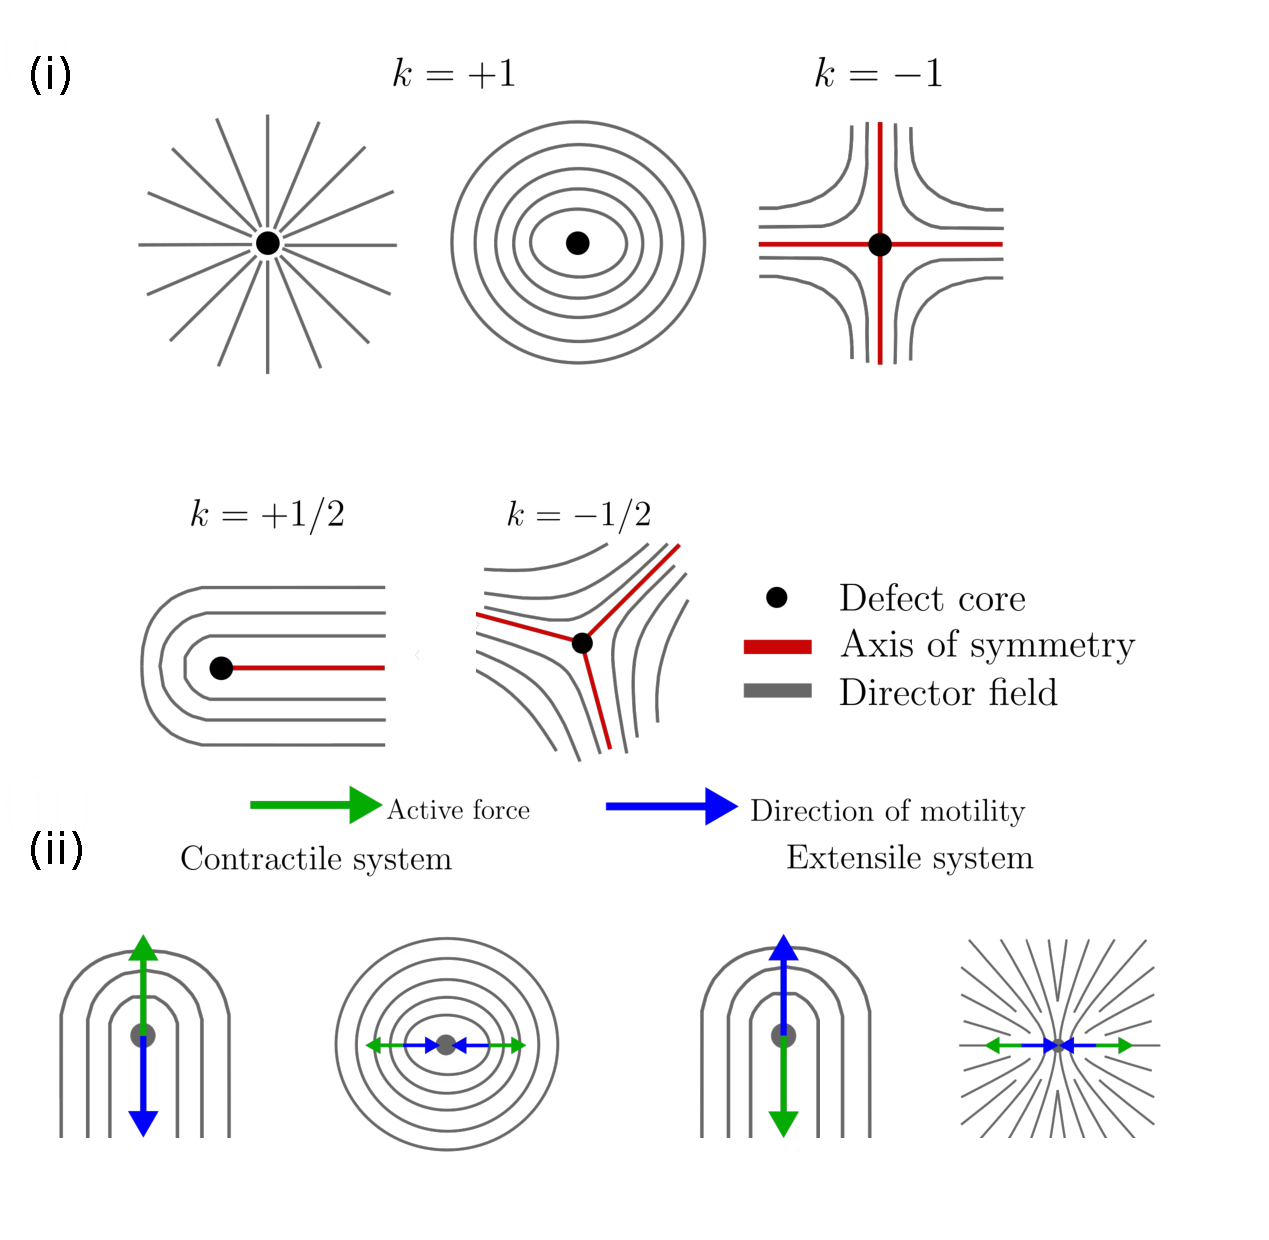
\includegraphics[width=0.8\textwidth]{chap_6_fig_2.pdf}
	\caption{ \textbf{Topological defects in active nematic surfaces.} (i) The charge of the topological defects is related to the number of axes of symmetry (red lines). (ii) Nature of active forces in a self-propelling $\textup{+} 1/2$ defect. Activity can induce a $\textup{+}1$ bound defect. Depending on the sign of activity, a vortex-type  or an aster-type bound defect is formed .}
	\label{fig_0_2}
\end{figure}
\begin{center}
	\begin{mybox}{gray}{\center{\textbf{Box B: Topological defects in active nematics}}}
		Topological defects  are (nearly) singular points with an abrupt gradient in the orientation field. Topological defects on a surface are classified based on their charge $k$ defined using the number of axes of symmetry $n$ as $k = 1 - \vert n/2\vert$ \cite{tang2017}.
		For example, as shown in Fig.~\ref{fig_0_2}, topological defects with $n=3$ and $n=1$ have a defect charge  of $k= \textup{+} 1/2$ and $k=\textup{-} 1/2$ respectively. In a passive nematic system, $\pm 1/2$ defects are stable. Activity renders a $\textup{+}1/2$ motile along its axis of symmetry, whereas due to its three-fold symmetry, a $\textup{-}1/2$ defect does not propel. Contractile (extensile) activity drives a $\textup{+}1/2$ defect in the direction of its tail (comet-head) \cite{thijssen2020,vafa2020}. As a result of activity-driven propulsion, two $\textup{+}1/2$ can overcome their repulsive force to create a bound $\textup{+}1$. For a contractile (an extensile) system, one then gets a $\textup{+}1$ defect with vortex-like (aster-like) structure \cite{thijssen2020, vafa2020}, see Fig.~\ref{fig_0_2}.
	\end{mybox}
\end{center}

For example, at the sub-cellular level, cytokinesis in the final stage of the cell cycle is triggered by the self-organization of a nematic bundle with a high density of actin filaments and bundling proteins in the equator, Fig.~\ref{fig_0}(i) \cite{anne2016, wollrab2016, leite2019}. As a result of this network organization, contractile forces are generated efficiently \cite{kelkar2020} leading to axial elongation  and furrowing in the cytoskeleton dividing a cell in two. A similar mechanism involving the self-organization of contractile rings has been shown to drive cellular deformations in notochord cells, Fig.~\ref{fig_0}(ii) \cite{Dong}, or wound closure after cell ablation, Fig.~\ref{fig_0}(iii) \cite{mandato2001}. %In contrast with the drastic shape changes driven by nematic contractile bundles, recent studies also indicate splitting of nematic tactoid (shown in Fig.~\ref{fig_0}(iv)) via a polarity sorting mechanism involving myosin-II gathering at the tactoids equator and sorting filaments into an aster that pinches the droplet \cite{weirich2017, brugues2014, kaznacheev2002}. 
Defect-modulated shape changes are observed in active nematic vesicles, Fig.~\ref{fig_0}(iv-v), where the motion of defects lead to filopodia-like protrusions. In smaller vesicles, a similar motion of defects leads to a spindle-like structure with two $+1$ defects at the ends of the spindle \cite{keber2014}. 


\begin{figure}[h!]
	\centering
	\includegraphics[width=1\textwidth]{chap_6_fig_1.pdf}
	\caption{ \textbf{Interplay between shape and nematic order at sub-cellular and supra-cellular scales.} (i) Cell division is achieved through the ingression of a dense bundle of contractile actomyosin 
		ring (white arrows) \cite{anne2016}. (ii) Contractile actomyosin ring (yellow arrows) drives constriction and elongation in Notochord cells \cite{Dong}. (iii) Cell wound healing driven by the constriction of a self-organized dense bundle of actomyosin ring around the ablated region \cite{mandato2001}. (iv) Transient shapes characterized by the formation of spikes around $\textup{+}1/2$ (top) and $\textup{+}1$ (bottom) defect sites in a layer of microtubules and kinesin motors in a lipid vesicle \cite{keber2014}. (v)  Morphologies of vesicles formed from nematic amphiphilic block copolymers  as a result of the interplay between nematic ordering and vesicle shape \cite{xing2012}. (vi) Hydra morphogenesis with defects acting as organizational centers. $\textup{+}1$ defect in the proximity of the mouth, the foot and the tip of each tentacle, and two $\textup{-}1/2$ defects at the base of each tentacle \cite{maroudas2021}. (vii) Mounds of myoblast cells protruding out of a $\textup{+}1$ nematic defect \cite{guillamat2020}.}
	\label{fig_0}
\end{figure}


In developing Hydra, an interplay between the nematic alignment of actin, biochemical signaling processes and topological constraints drives morphogenesis, Fig.~\ref{fig_0}(vi) \cite{maroudas2021}. In particular, $+1$ topological defects in Hydra tissue spheroids act as precursors to the development of head/foot, whereas ${\text +}1/2$ defects appear at the base of an early bud, with a $+1$ defect at its tip, as the bud protrudes to form a tentacle. At the supra-cellular level, defect-mediated morphogenesis has been observed in myoblasts cultures  that form cylindrical  multi-cellular  protrusions around spiral- and aster-type topological defects, Fig.~\ref{fig_0}(vii) \cite{guillamat2020}.



The non-trivial relationship between the out-of-equilibrium flows, nemato-dynamics, curvature and topological constraints has been widely explored theoretically and computationally on nearly rigid surfaces, a situation that can be justified by high surface tension or by the presence of  a confining rigid bulk medium  \cite{ellis2018}. These studies have been performed on surfaces such as cylinders \cite{napoli2020, pearce2020}, spheres and prolate/oblate spheroids \cite{nestler2018, torres2020, henkes2017, zhang2020, keber2014, vcopar2019,alaimo2017, ehrig2017,khoromskaia2017,kralj2011}, tori \cite{torres2020, ellis2018}, and nonic surfaces \cite{nestler2018}. These studies show that a genus-zero surface self-organizes defects with a total topological charge of $+2$, following the Poincare-Brouwer theorem \cite{kamien2002}. In the absence of activity, these defects achieve steady low-energy configurations. In a sphere, such configuration is characterized by a  tetrahedral arrangement of defect with an average inter-defect angle of $109.5^{\circ}$, whereas on an ellipsoid defects arrange at the poles \cite{nitschke2020}. The energetic cost of a defect on the surface depends on the local Gaussian curvature \cite{nestler2018, ellis2018}. When activity goes above a critical threshold, these defects become mobile and undergo oscillations between low and high energy configurations. At larger activities, the topological defects enter a regime of irregular and chaotic motion, often accompanied by spontaneous proliferation and annihilation of defects, a regime  called active turbulence \cite{ellis2018,vcopar2019,gao2017}. 

The theoretical models used to study these dynamics can be broadly classified in two approaches: 1) The first approach is based on particle simulations \cite{alaimo2017, ehrig2017,keber2014,khoromskaia2017,ellis2018}, which involves sets of  ordinary differential equations  governing particle positions and orientations. %(ODEs). The first ODE governs the position of the particles accounting for spontaneous directed propulsion due to activity along with repulsive and attractive forces between the particles depending on their topological charge. The second ODE governs the orientation of the active particle accounting for the torque acting on it due to the tendency of particles to align with the neighbours as well as with the direction of its velocity. The coupled ODEs are integrated numerically using standard Euler or Runge-Kutta methods. 
2) In the second approach involves a mean-field continuum description of the dynamics of orientational order and and flow in terms of partial differential equations on a curved surface \cite{vcopar2019,torres2020,zhang2020, napoli2020,pearce2020,nestler2018}. In this approach, the governing equations are solved using the Lattice-Boltzman algorithm \cite{denniston2004} or space discretization schemes based on the finite element method \cite{nestler2018}. 

Shape changes resulting from the interwoven coupling between nematic order, geometric parameters, topological constraints and active hydrodynamics have been explored in fewer studies  \cite{al2021}. \citet{nitschke2020} proposed a thermodynamically consistent mathematical model for the relaxation dynamics of a passive nematic system on a deformable surface. In this model, the free-energy consists of the Helfrich energy, the Landau-de Gennes energy and a surface-area penalization energy.  The numerical formulation is an extension of \cite{nitschke2019}, which was used to study shape evolving surfaces with polar order. They show an interesting interplay between defect configurations and intrinsic/extrinsic curvature contributions. \citet{xing2012} also studied the relationship between the morphology of a passive vesicle and surface nematic order. The study involves a minimalistic mathematical model with the Helfrich energy and a potential similar to the Landau-de Gennes energy that only penalizes the gradients in the orientation field. It is shown that in the limit where the contribution of the Landau-de Gennes energy is far greater than the Helfrich energy, the ground state of a vesicle with spherical topology is a faceted tetrahedron, with $+1/2$ defects located at each of the four corners. On the other hand, in the limit where the relative contribution of Helfrich energy is higher, the ground state is an infinitesimally deformed spherical vesicle with a tetrahedral defect configuration. None of the above-mentioned studies account for the dissipation involved in surface flows nor for activity. 

Recently,  \citet{vafa2021} have proposed a minimal framework for active surfaces coupling frictional flows, nematic order, shape and density. However, other possibly relevant ingredients such as shear dissipation, the dissipative coupling between flow and nematic order and Helfrich energy are not accounted for. Consistent with experimental findings \cite{kawaguchi2017,maroudas2021}, the numerical solution of the model demonstrates that (i)  cell density increases (decreases) at plus (minus) defects, (ii) curvature  is positive (negative) near a plus (minus) defect and (iii) activity can stabilize a ring configuration of equally spaced $\textup{+}1$ defects separated by pairs of $\textup{-}1/2$ defects. \citet{metselaar2019} and \citet{https://doi.org/10.48550/arxiv.2205.06805} have employed more comprehensive active nematic surface models to simulate defect-mediated morphogenesis. The model accounts for orientational order, shape dynamics, surface Stokes flow as well as active tensions. Hybrid lattice-Boltzmann numerical simulations are used to explore the mechanism behind shape changes directed by self-organized topological defects and active flows. \citet{Ruske2021} proposed a theoretical and computational framework to study a related problem in interfacial active nematics, the reshaping of active droplets in 3D, which exhibit in-plane and out-of-plane nematic order at the interface. The proposed governing equations are solved using a hybrid lattice-Boltzmann finite-difference method. %The numerical experiments  show that active stresses cause in-plane (in extensile droplet) and out-of-plane (in contractile droplet)  alignment of the director field at the interface of droplets. This `active anchoring' results from an interplay between active flows and a change in nematic orientation. Such gradient in nematic direction trigger the formation of fingerlike protrusions (in extensile droplets) and surface wrinkles and droplet invagination (in contractile droplets). 

Despite recent efforts, there are two obstacles to study the multiphysics and geometry-dependent mechanics of active and deformable fluid nematic surfaces. The first obstacle involves the need for a general theoretical framework for such a complex system. In the existing literature,  theories for active surfaces have been proposed, which can potentially address this challenge. These frameworks involve two major approaches: (i) The first approach \cite{salbreux2022} is a generic framework for active surfaces and involves identifying the forces and moments acting on a surface to formulate the  governing equations encoding balance of momentum and generalized forces. The calculation of rate-of-change of free-energy identifies the conjugate pairs of thermodynamic forces and fluxes. Lastly, the relationship between conjugate pairs is postulated in terms of linear constitutive laws that satisfy the Onsager relations. (ii) The second approach \cite{torres2019, arroyo2018} is based on Onsager's variational formalism, where the constitutive relationships are implicit in the form of free-energy, dissipative potentials and activity functionals. The governing equations follow from a minimization principle where free-energy release rate, dissipation and activity compete. 

The second obstacle involves the lack of an efficient computation framework to solve resulting Euler-Lagrange equations. The literature on numerical methods for such tensor-valued problems is rare and mainly restricted to the sphere. Here a major difficulty is the approximation of tensor fields such as the nematic field $\bm{q}$ on general surfaces. To address this, \citet{torres2020} proposed a Local Monge parametrization to interpolate  higher-order tensors on arbitrary surfaces. Alternatively, it is possible to interpolate bulk tensors and impose with a penalty the constraint that they should be tangential to the surface \cite{nestler2018,metselaar2019,https://doi.org/10.48550/arxiv.2205.06805}, at the expense of additional degrees of freedom and a stiff term in the equations. 


In the next chapters, we fill this gap by proposing a theoretical framework based on Onsager's variational formalism for active nematic deformable fluid surfaces. This variational method naturally lends itself to finite element discretizations to numerically discretize  the governing equations in space. Furthermore, Onsager's formalism admits a time-incremental variational principle that serves as a time-discretization method and inherits the built-it thermodynamic consistency and nonlinear stability of the time-continuous version. This means that in the absence of power input, the free-energy is a Lyapunov functional of the dynamics. In Chapter~\ref{chap_7}, we formulate the mathematical model, derive the strong form of the coupled equations governing shape dynamics and nemato-hydrodyamics, and interpret these equations. In Chapter~\ref{chap_8}, we focus on the application of the general model to the actin cytoskeleton, and more specifically, to the assembly of the cytokinetic ring leading to cell division. In this model, the surface is compressible and density effects are crucial. We restrict the model to axisymmetry and develop an efficient finite element numerical approach. In Chapter~\ref{chap_9}, we focus on inextensible active liquid crystal nematic vesicles in a fully 3D setting, and propose a general finite element method for active nematic and deformable fluid surfaces. 

